\documentclass[a4paper]{report}
\usepackage[utf8]{inputenc}
\usepackage[T1]{fontenc}
\usepackage{RJournal}
\usepackage{amsmath,amssymb,array}
\usepackage{booktabs}
\usepackage{longtable}
\usepackage{calc}

\providecommand{\tightlist}{%
  \setlength{\itemsep}{0pt}\setlength{\parskip}{0pt}}



\usepackage{mathrsfs}
\newcommand{\defeq}{\stackrel{\tiny def}{=}}
\newcommand{\fct}[1]{\texttt{\detokenize{#1}()}}
\usepackage{pdflscape}

\begin{document}

\sectionhead{Contributed research article supplement}
\volume{XX}
\volnumber{YY}
\year{20ZZ}
\month{AAAA}


\begin{article}
\title{Supplementary Materials for ldmppr: Location Dependent Marked Point Processes in R}


\author{by Lane Drew and Andee Kaplan}

\maketitle

\appendix

\section{Additional details on initialization defaults for \\ \texttt{\detokenize{estimate_process_parameters}()}}\label{appA}

We initialize self-correcting model parameters using data-adaptive
heuristics designed to place the optimizer in a stable region of the
parameter space. The baseline log-intensity is anchored by the empirical
event rate via \(\alpha_{\text{base}} = \log(n / \Delta t)\). The
self-correction strength \(\gamma_1\) is initialized on a conservative
\(\log(n) / n\)-type scale to reduce unstable behavior early in
optimization. To capture monotone temporal trends, \(\beta_1\) is
initialized from a Poisson regression of binned event counts on time
(with an offset for bin width), with a fallback that induces a modest
multiplicative change across the observation window.

Spatial inhibition range \(\alpha_2\) is initialized using the median
nearest-neighbor distance (or a conservative geometric fallback).
Spatio-temporal interaction scales are bounded by the observation
window: the spatial scale parameter is capped by the window diagonal,
and the temporal interaction scale is capped by the observed time span
(equal to 1 under the default time mapping). These choices provide
stable starting values and natural finite bounds for optimization.

\section{Stage-wise runtime benchmarks}\label{appB}

To quantify fitting cost, we benchmarked runtime for
\texttt{\detokenize{estimate_process_parameters}()} and
\texttt{\detokenize{train_mark_model}()} on three contiguous datasets:
(i) \texttt{medium\_example\_data}, (ii) a contiguous window with
approximately 200 points, and (iii) a contiguous window with
approximately 400 points. The larger datasets were selected as
contiguous windows from the full domain (rather than random point
subsamples) to preserve local dependence structure.

Stage-wise timing artifacts can be regenerated by running: \newline
\texttt{LDMPPR\_STAGE\_PROFILE=full} \newline
\texttt{LDMPPR\_STAGE\_REPS=10} \newline
\texttt{LDMPPR\_STAGE\_CORES=1,7} \newline
\texttt{LDMPPR\_STAGE\_DATASETS=medium,win200,win400} \newline
\texttt{Rscript "scripts/supplement\_stage\_timing\_study.R"}.

If \texttt{LDMPPR\_RASTER\_DIR} is not set, required external rasters
are downloaded automatically from ESS-DIVE into
\texttt{data/ess\_dive\_rasters}.

\begin{longtable}[]{@{}
  >{\raggedright\arraybackslash}p{(\linewidth - 20\tabcolsep) * \real{0.0833}}
  >{\raggedleft\arraybackslash}p{(\linewidth - 20\tabcolsep) * \real{0.0729}}
  >{\raggedleft\arraybackslash}p{(\linewidth - 20\tabcolsep) * \real{0.1250}}
  >{\raggedleft\arraybackslash}p{(\linewidth - 20\tabcolsep) * \real{0.0625}}
  >{\raggedleft\arraybackslash}p{(\linewidth - 20\tabcolsep) * \real{0.0521}}
  >{\raggedleft\arraybackslash}p{(\linewidth - 20\tabcolsep) * \real{0.1042}}
  >{\raggedleft\arraybackslash}p{(\linewidth - 20\tabcolsep) * \real{0.0833}}
  >{\raggedleft\arraybackslash}p{(\linewidth - 20\tabcolsep) * \real{0.1146}}
  >{\raggedleft\arraybackslash}p{(\linewidth - 20\tabcolsep) * \real{0.0938}}
  >{\raggedleft\arraybackslash}p{(\linewidth - 20\tabcolsep) * \real{0.1146}}
  >{\raggedleft\arraybackslash}p{(\linewidth - 20\tabcolsep) * \real{0.0938}}@{}}
\caption{Stage-wise runtime summary (seconds): process estimation and
mark-model training.}\tabularnewline
\toprule\noalign{}
\begin{minipage}[b]{\linewidth}\raggedright
Dataset
\end{minipage} & \begin{minipage}[b]{\linewidth}\raggedleft
Points
\end{minipage} & \begin{minipage}[b]{\linewidth}\raggedleft
Window Side
\end{minipage} & \begin{minipage}[b]{\linewidth}\raggedleft
Cores
\end{minipage} & \begin{minipage}[b]{\linewidth}\raggedleft
Runs
\end{minipage} & \begin{minipage}[b]{\linewidth}\raggedleft
Est. Mean
\end{minipage} & \begin{minipage}[b]{\linewidth}\raggedleft
Est. SD
\end{minipage} & \begin{minipage}[b]{\linewidth}\raggedleft
Train Mean
\end{minipage} & \begin{minipage}[b]{\linewidth}\raggedleft
Train SD
\end{minipage} & \begin{minipage}[b]{\linewidth}\raggedleft
Total Mean
\end{minipage} & \begin{minipage}[b]{\linewidth}\raggedleft
Total SD
\end{minipage} \\
\midrule\noalign{}
\endfirsthead
\toprule\noalign{}
\begin{minipage}[b]{\linewidth}\raggedright
Dataset
\end{minipage} & \begin{minipage}[b]{\linewidth}\raggedleft
Points
\end{minipage} & \begin{minipage}[b]{\linewidth}\raggedleft
Window Side
\end{minipage} & \begin{minipage}[b]{\linewidth}\raggedleft
Cores
\end{minipage} & \begin{minipage}[b]{\linewidth}\raggedleft
Runs
\end{minipage} & \begin{minipage}[b]{\linewidth}\raggedleft
Est. Mean
\end{minipage} & \begin{minipage}[b]{\linewidth}\raggedleft
Est. SD
\end{minipage} & \begin{minipage}[b]{\linewidth}\raggedleft
Train Mean
\end{minipage} & \begin{minipage}[b]{\linewidth}\raggedleft
Train SD
\end{minipage} & \begin{minipage}[b]{\linewidth}\raggedleft
Total Mean
\end{minipage} & \begin{minipage}[b]{\linewidth}\raggedleft
Total SD
\end{minipage} \\
\midrule\noalign{}
\endhead
\bottomrule\noalign{}
\endlastfoot
medium & 106 & 50 & 1 & 10 & 2.91 & 0.33 & 23.34 & 0.76 & 26.25 &
0.74 \\
medium & 106 & 50 & 7 & 10 & 2.23 & 0.27 & 23.76 & 0.15 & 25.99 &
0.28 \\
win200 & 207 & 75 & 1 & 10 & 7.72 & 1.09 & 36.05 & 0.16 & 43.76 &
1.14 \\
win200 & 207 & 75 & 7 & 10 & 4.77 & 0.79 & 35.45 & 0.19 & 40.22 &
0.72 \\
win400 & 413 & 100 & 1 & 10 & 19.95 & 1.87 & 60.20 & 0.52 & 80.15 &
1.82 \\
win400 & 413 & 100 & 7 & 10 & 7.74 & 2.02 & 60.08 & 0.29 & 67.82 &
2.06 \\
\end{longtable}

Using one core, process-estimation time increases from 2.91s (n=106) to
19.95s (n=413), while mark-model training increases from 23.34s to
60.20s over the same range.

\section{Simulation-check runtime benchmarks}\label{appC}

We benchmarked runtime for \texttt{\detokenize{check_model_fit}()} using
\texttt{n\_sim} values of 200, 500, 1000, and 2500, with fixed seeds and
matched settings otherwise. This isolates simulation-based
goodness-of-fit cost and provides practical guidance for exploratory
versus final checks.

Simulation-check timing artifacts can be regenerated by running:
\newline \texttt{LDMPPR\_TIMING\_MODE=full} \newline
\texttt{LDMPPR\_TIMING\_N\_SIM=200,500,1000,2500} \newline
\texttt{LDMPPR\_TIMING\_REPS=10} \newline
\texttt{LDMPPR\_TIMING\_CORES=1,2} \newline
\texttt{Rscript "scripts/supplement\_sim\_timing\_study.R"}.

\begin{longtable}[]{@{}
  >{\raggedleft\arraybackslash}p{(\linewidth - 10\tabcolsep) * \real{0.1690}}
  >{\raggedleft\arraybackslash}p{(\linewidth - 10\tabcolsep) * \real{0.0845}}
  >{\raggedleft\arraybackslash}p{(\linewidth - 10\tabcolsep) * \real{0.0704}}
  >{\raggedleft\arraybackslash}p{(\linewidth - 10\tabcolsep) * \real{0.1831}}
  >{\raggedleft\arraybackslash}p{(\linewidth - 10\tabcolsep) * \real{0.1549}}
  >{\raggedleft\arraybackslash}p{(\linewidth - 10\tabcolsep) * \real{0.3380}}@{}}
\caption{Runtime summary (seconds) for simulation-based model
checking.}\tabularnewline
\toprule\noalign{}
\begin{minipage}[b]{\linewidth}\raggedleft
Simulations
\end{minipage} & \begin{minipage}[b]{\linewidth}\raggedleft
Cores
\end{minipage} & \begin{minipage}[b]{\linewidth}\raggedleft
Runs
\end{minipage} & \begin{minipage}[b]{\linewidth}\raggedleft
Elapsed Mean
\end{minipage} & \begin{minipage}[b]{\linewidth}\raggedleft
Elapsed SD
\end{minipage} & \begin{minipage}[b]{\linewidth}\raggedleft
Combined \(p\)-value Mean
\end{minipage} \\
\midrule\noalign{}
\endfirsthead
\toprule\noalign{}
\begin{minipage}[b]{\linewidth}\raggedleft
Simulations
\end{minipage} & \begin{minipage}[b]{\linewidth}\raggedleft
Cores
\end{minipage} & \begin{minipage}[b]{\linewidth}\raggedleft
Runs
\end{minipage} & \begin{minipage}[b]{\linewidth}\raggedleft
Elapsed Mean
\end{minipage} & \begin{minipage}[b]{\linewidth}\raggedleft
Elapsed SD
\end{minipage} & \begin{minipage}[b]{\linewidth}\raggedleft
Combined \(p\)-value Mean
\end{minipage} \\
\midrule\noalign{}
\endhead
\bottomrule\noalign{}
\endlastfoot
200 & 1 & 10 & 4.33 & 0.10 & 0.133 \\
200 & 2 & 10 & 4.08 & 0.17 & 0.136 \\
500 & 1 & 10 & 10.63 & 0.13 & 0.136 \\
500 & 2 & 10 & 9.43 & 0.19 & 0.146 \\
1000 & 1 & 10 & 21.79 & 0.16 & 0.215 \\
1000 & 2 & 10 & 19.37 & 0.72 & 0.151 \\
2500 & 1 & 10 & 52.74 & 0.35 & 0.227 \\
2500 & 2 & 10 & 49.21 & 0.44 & 0.217 \\
\end{longtable}

At one core, mean check time grows from 4.33s at n\_sim=200 to 52.74s at
n\_sim=2500.

For the largest run (n\_sim=2500), moving from one core to two cores
reduces mean wall-clock time by 6.7\%.

For iterative model development, moderate simulation counts can reduce
turnaround time. For final reporting, larger simulation counts provide
more stable Monte Carlo \(p\)-value estimates.

For a direct, reproducible benchmark of the improved paper workflow
(estimation + mark-model training + model check, matching the script in
the main paper), run: \newline \texttt{LDMPPR\_BENCH\_REPS=10} \newline
\texttt{Rscript "scripts/benchmark\_improved\_workflow\_timing.R"}.

\section{Description and interpretation of the \texttt{spatstat} comparison framework}\label{appD}

The comparison script \texttt{scripts/spatstat\_comp.R} implements a
two-stage baseline intended to approximate the improved manuscript
workflow as closely as possible while utilizing the \texttt{spatstat}
modeling framework:

\begin{enumerate}
\item A spatial point process is fit with \texttt{spatstat::ppm}, using raster-derived covariates and a Strauss interaction term for regularity/inhibition.
\item A separate XGBoost mark model is fit from location/raster features with optional competition-index features. To align with the improved paper workflow, tuning uses MAE with 10-fold cross-validation and a tuning grid size of 150.
\item Simulated spatial patterns from the fitted \texttt{ppm} model are marked using the fitted XGBoost model then evaluated with the same LGFJEV and combined GET-rank envelope machinery used in the package-facing checks.
\end{enumerate}

For the direct comparison below we use \texttt{n\_sim = 2500} for both
methods, matching the improved-paper model-check setting. For the
\texttt{ldmppr} workflow, we match the paper's specifications exactly:
estimation and model-check steps run without parallelization, while
mark-model training uses \texttt{parallel = TRUE}. Comparison artifacts
can be regenerated by running: \newline
\texttt{LDMPPR\_COMP\_N\_SIM=2500} \newline
\texttt{LDMPPR\_COMP\_PARALLEL=true} \newline
\texttt{Rscript "scripts/ldmppr\_comp\_timing.R"} and \newline
\texttt{LDMPPR\_SPATSTAT\_N\_SIM=2500} \newline
\texttt{LDMPPR\_SPATSTAT\_CV\_FOLDS=10} \newline
\texttt{LDMPPR\_SPATSTAT\_TUNING\_GRID=150} \newline
\texttt{LDMPPR\_SPATSTAT\_FG\_CORRECTION=km} \newline
\texttt{LDMPPR\_SPATSTAT\_PARALLEL=true} \newline
\texttt{LDMPPR\_SPATSTAT\_NUM\_CORES=7} \newline
\texttt{Rscript "scripts/spatstat\_comp.R"}.

If \texttt{LDMPPR\_RASTER\_DIR} is not set, required external rasters
are downloaded automatically from ESS-DIVE into
\texttt{data/ess\_dive\_rasters}.

\begin{longtable}[]{@{}
  >{\raggedright\arraybackslash}p{(\linewidth - 10\tabcolsep) * \real{0.2603}}
  >{\raggedleft\arraybackslash}p{(\linewidth - 10\tabcolsep) * \real{0.1644}}
  >{\raggedleft\arraybackslash}p{(\linewidth - 10\tabcolsep) * \real{0.1233}}
  >{\raggedleft\arraybackslash}p{(\linewidth - 10\tabcolsep) * \real{0.1370}}
  >{\raggedleft\arraybackslash}p{(\linewidth - 10\tabcolsep) * \real{0.1370}}
  >{\raggedleft\arraybackslash}p{(\linewidth - 10\tabcolsep) * \real{0.1781}}@{}}
\caption{Side-by-side timing and combined \(p\)-value comparison (ldmppr
vs spatstat two-stage) for \(n = 2500\) simulations in
seconds.}\tabularnewline
\toprule\noalign{}
\begin{minipage}[b]{\linewidth}\raggedright
Method
\end{minipage} & \begin{minipage}[b]{\linewidth}\raggedleft
Process fit
\end{minipage} & \begin{minipage}[b]{\linewidth}\raggedleft
Mark fit
\end{minipage} & \begin{minipage}[b]{\linewidth}\raggedleft
Check fit
\end{minipage} & \begin{minipage}[b]{\linewidth}\raggedleft
Total (s)
\end{minipage} & \begin{minipage}[b]{\linewidth}\raggedleft
Combined \(p\)
\end{minipage} \\
\midrule\noalign{}
\endfirsthead
\toprule\noalign{}
\begin{minipage}[b]{\linewidth}\raggedright
Method
\end{minipage} & \begin{minipage}[b]{\linewidth}\raggedleft
Process fit
\end{minipage} & \begin{minipage}[b]{\linewidth}\raggedleft
Mark fit
\end{minipage} & \begin{minipage}[b]{\linewidth}\raggedleft
Check fit
\end{minipage} & \begin{minipage}[b]{\linewidth}\raggedleft
Total (s)
\end{minipage} & \begin{minipage}[b]{\linewidth}\raggedleft
Combined \(p\)
\end{minipage} \\
\midrule\noalign{}
\endhead
\bottomrule\noalign{}
\endlastfoot
ldmppr & 7.49 & 136.54 & 53.84 & 197.87 & 0.2819 \\
spatstat two-stage & 0.02 & 128.59 & 443.81 & 443.81 & 0.0016 \\
\end{longtable}

Under matched comparison settings (n\_sim=2500), the combined GET
\(p\)-value is 0.2819 for ldmppr and 0.0016 for the two-stage spatstat
baseline.

Total runtime is 197.87s for ldmppr versus 443.81s for the two-stage
spatstat baseline; in the table above, the spatstat check time reports
simulation plus envelope-check computation, while the ldmppr check time
reports the corresponding integrated model-check step.

\begin{longtable}[]{@{}lrr@{}}
\caption{Side-by-side \(p\)-values by summary function, including the
combined test \(p\)-value.}\tabularnewline
\toprule\noalign{}
Statistic & ldmppr \(p\)-value & spatstat two-stage \(p\)-value \\
\midrule\noalign{}
\endfirsthead
\toprule\noalign{}
Statistic & ldmppr \(p\)-value & spatstat two-stage \(p\)-value \\
\midrule\noalign{}
\endhead
\bottomrule\noalign{}
\endlastfoot
L & 0.4650 & 0.0144 \\
F & 0.0728 & 0.5614 \\
G & 0.7137 & 0.1236 \\
J & 0.1443 & 0.0324 \\
E & 0.0688 & 0.0140 \\
V & 0.9100 & 0.0024 \\
Combined & 0.2819 & 0.0016 \\
\end{longtable}

At the 0.05 level, ldmppr shows significant departures for: none. The
two-stage spatstat baseline shows significant departures for: L, J, E,
V.

\begin{landscape}


\begin{center}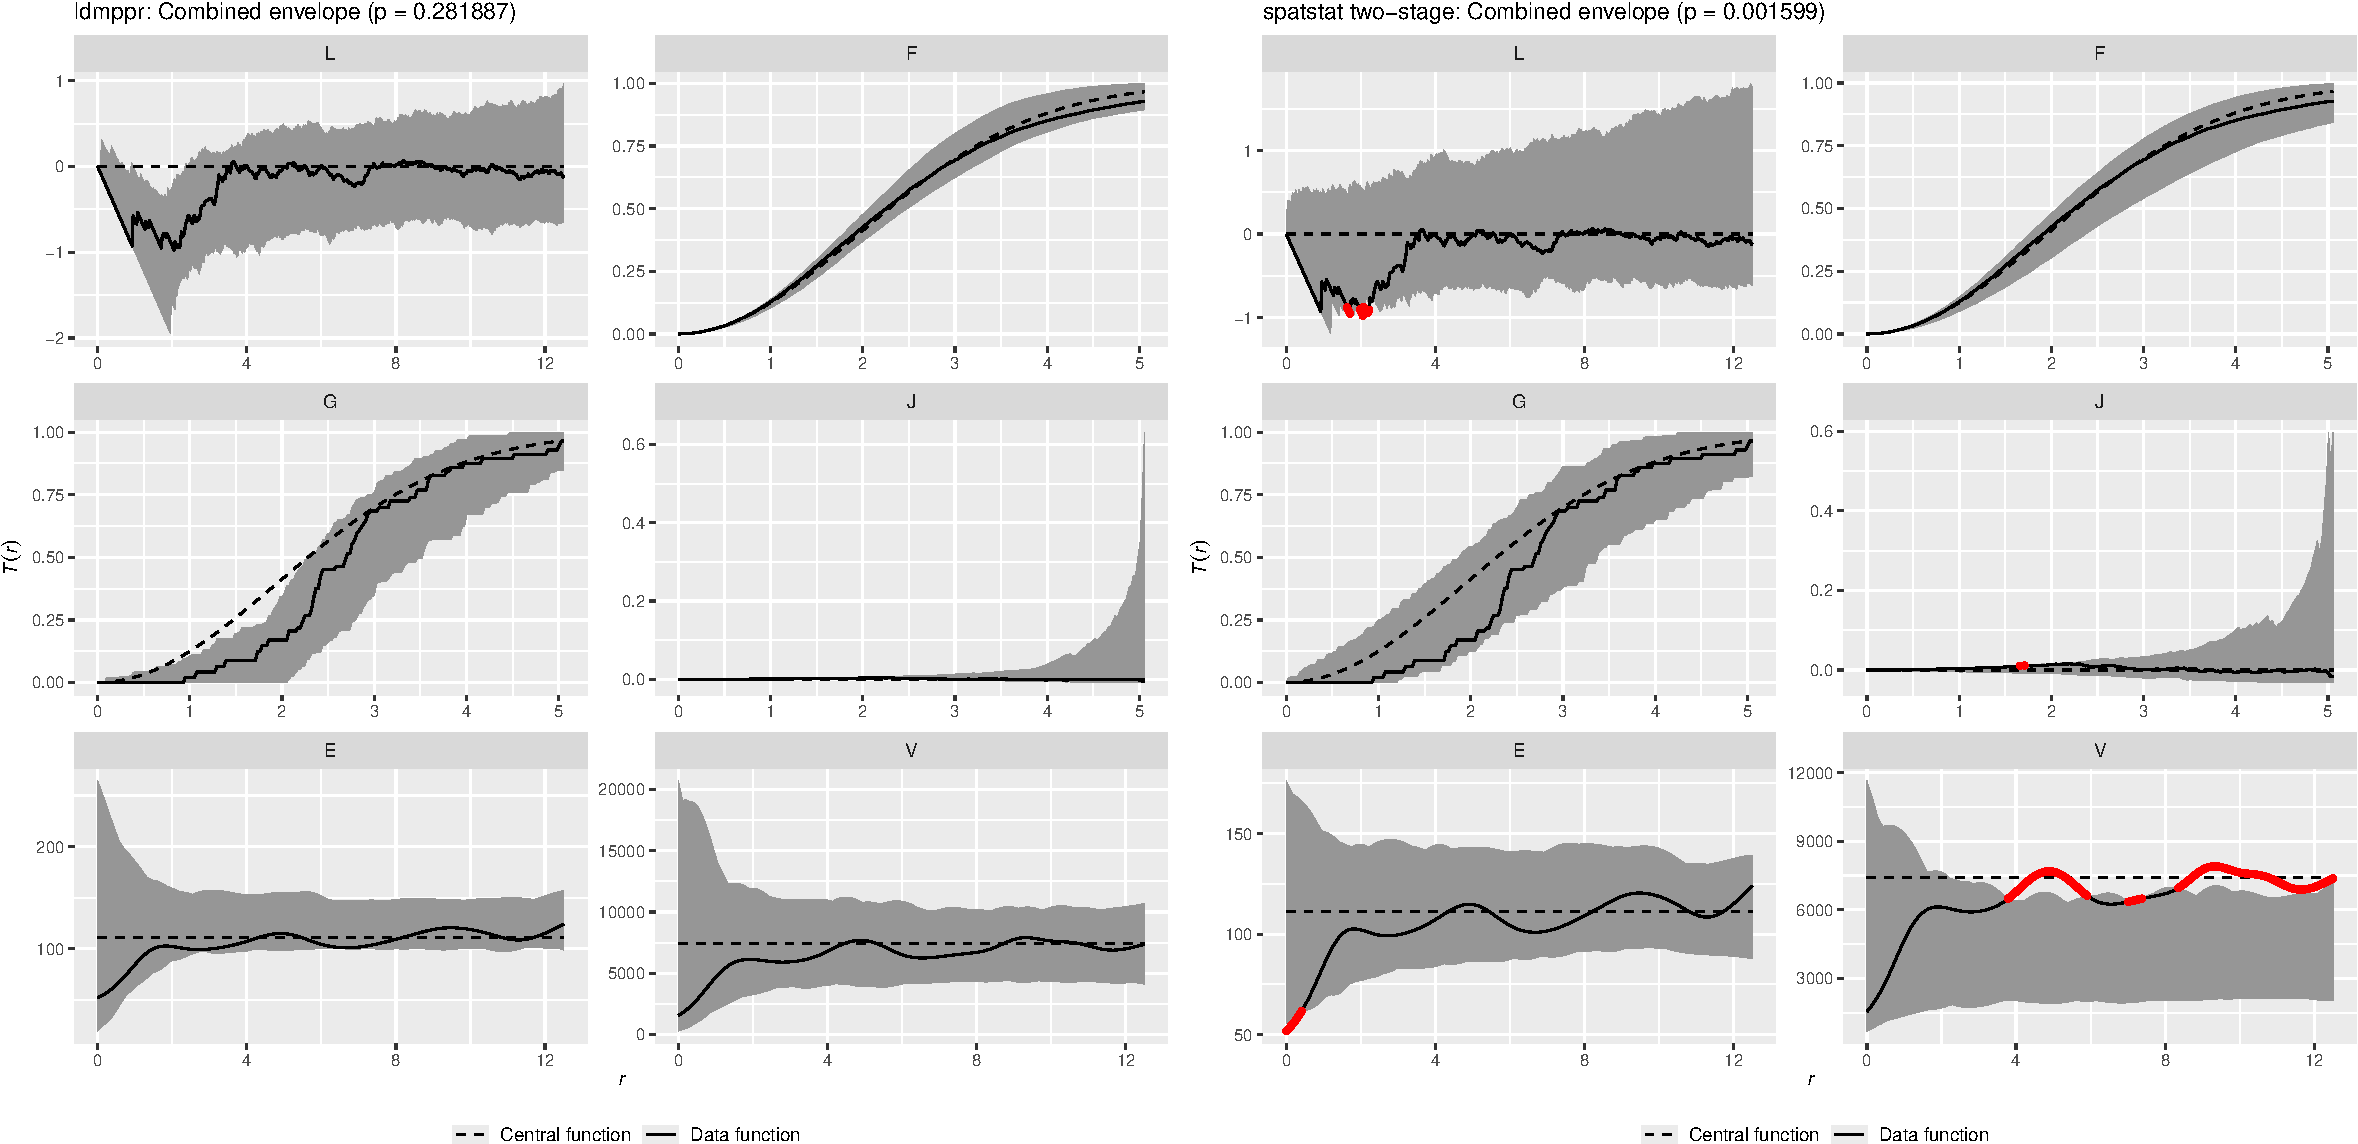
\includegraphics[width=1\linewidth]{ldmppr_supplement_files/figure-latex/comp_check_plots-1} \end{center}

\end{landscape}

\begin{center}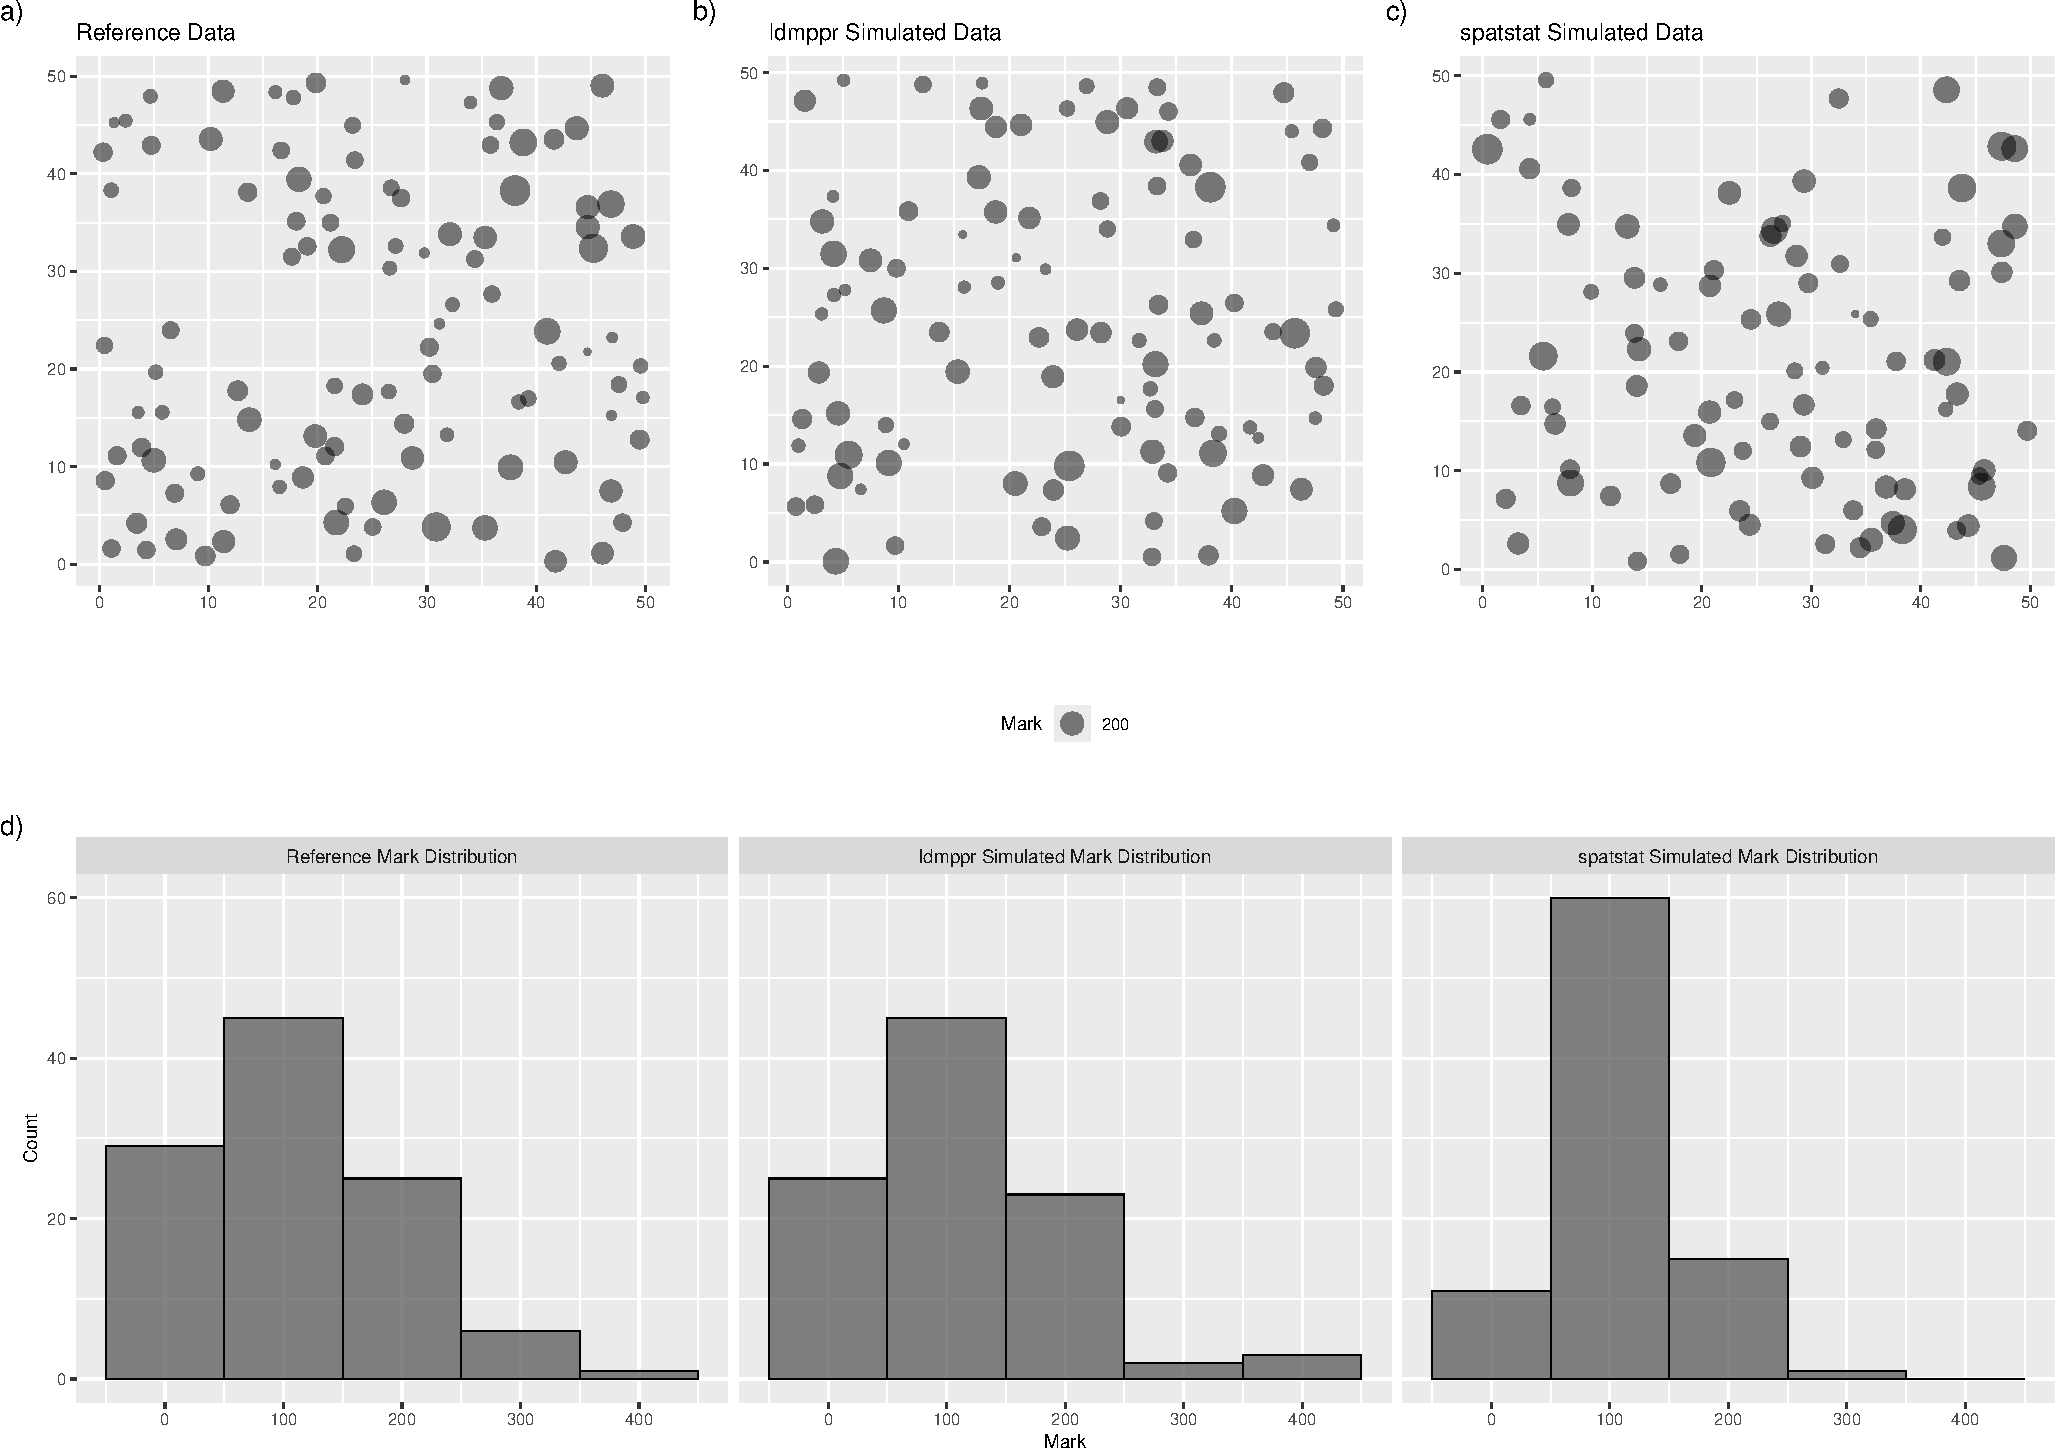
\includegraphics[width=1\linewidth]{ldmppr_supplement_files/figure-latex/comp_data_plots-1} \end{center}

This baseline provides useful context but is not a fully comparable
benchmark for the mechanistic \texttt{ldmppr} workflow. In particular,
temporal/self-correcting dynamics are not estimated in a single unified
model, and mark generation is modularized as a second stage. We
therefore interpret these results as contextual sensitivity evidence
rather than a definitive head-to-head comparison.

\end{article}

\end{document}
